\documentclass[12pt]{article}

\usepackage{sbc-template}
\usepackage{graphicx,url}
\usepackage[utf8]{inputenc}
\usepackage[brazil]{babel}
\usepackage[latin1]{inputenc}  

     
\sloppy

\title{Instructions for Authors of SBC Conferences\\ Papers and Abstracts}

\author{Luciana P. Nedel\inst{1}, Rafael H. Bordini\inst{2}, Flávio Rech
  Wagner\inst{1}, Jomi F. Hübner\inst{3} }


\address{Instituto de Informática -- Universidade Federal do Rio Grande do Sul
  (UFRGS)\\
  Caixa Postal 15.064 -- 91.501-970 -- Porto Alegre -- RS -- Brazil
\nextinstitute
  Department of Computer Science -- University of Durham\\
  Durham, U.K.
\nextinstitute
  Departamento de Sistemas e Computação\\
  Universidade Regional de Blumenal (FURB) -- Blumenau, SC -- Brazil
  \email{\{nedel,flavio\}@inf.ufrgs.br, R.Bordini@durham.ac.uk,
  jomi@inf.furb.br}
}

\begin{document} 

\maketitle

\begin{abstract}
  This meta-paper describes the style to be used in articles and short papers
  for SBC conferences. For papers in English, you should add just an abstract
  while for the papers in Portuguese, we also ask for an abstract in
  Portuguese (``resumo''). In both cases, abstracts should not have more than
  10 lines and must be in the first page of the paper.
\end{abstract}
     
\begin{resumo} 
  Este meta-artigo descreve o estilo a ser usado na confecção de artigos e
  resumos de artigos para publicação nos anais das conferências organizadas
  pela SBC. É solicitada a escrita de resumo e abstract apenas para os artigos
  escritos em português. Artigos em inglês deverão apresentar apenas abstract.
  Nos dois casos, o autor deve tomar cuidado para que o resumo (e o abstract)
  não ultrapassem 10 linhas cada, sendo que ambos devem estar na primeira
  página do artigo.
\end{resumo}



\section{Introduction}
\label{sec:intro}

%******* Introduction of the Dash technology and Cloud/Fog networks****
Com o surgimento de populares serviços de streaming de vídeo, atualmente, esses conteúdos multimídia são fornecidos a uma infinidade de heterogêneos dispositivos, de telefones celulares a TVs. Onde uma transmissão de video suave possui diferentes e rigorosos requisitos, como um canal de comunicação de boa qualidade bem como um fluxo constante e ininterrupto de informações~\cite{Immich2018WinNet}. Para acomodar essa demanda, bem como manter uma boa Qualidade de Experiencia~(\textit{Quality of Experience} - QoE) do usuário, grandes players como Microsoft, Apple, Adobe e Netflix adotam o paradigma Transmissão Adaptativa HTTP~(\textit{HTTP Adaptive Streaming} - HAS)~\cite{company:dashs}. Hoje, esse tráfego multimídia HAS corresponde à maior parte dos dados que circulam pela Internet em todo o mundo, com previsão de crescimento nos próximos anos. Eles são decompostos essencialmente em Servidores HTTP para atender essa demanda crescente.


% ----------------------------------------------------------------------------
% What is the current context in mobile network in terms of traffic and users? 
% ----------------------------------------------------------------------------

%The purpose of these schemes is to ensure a high QoE for users in the presence of fluctuations in bandwidth due to some factors such as network congestion control, signal strength, packet loss and so on. Although these fluctuations are quite common on the public Internet, they can also occur in private networks, such as home networks or even managed networks, where there is usually admission control and different QoS tools are used.

% ----------------------------------------------------------------------------
% What carries have been doing to address the increasing traffic?
% ----------------------------------------------------------------------------

Today, traditional video streaming services such as Content Distribution Networks~(CDN) and proxy are designed to deliver multimedia content across large cloud data centers. These cloud systems typically use a set of servers where traffic passes through the core of the network. Also, devices are generally connected by static users and stable internet links~\cite{sitaraman:ACD2014}. In this way, creating these systems partially solves the problems of scalability, availability and interoperability, but at the same time presents new challenges~(for example, higher latency and congestion of the core network)~\cite{tran:wons17,ye:ITC17, taleb:JSAC18}. Several works in the literature highlight fog/edge computing to handle the new video traffic demands that are emerging. Where data centers with less processing and storage capacity can provide services/virtualization closer to the end user. Thus, the edge of the network can provide latency rates that the cloud cannot otherwise achieve~\cite{gamaUCC2019, rosarioSENSORS2018}.

Although many research papers address streaming video services in conjunction with fog/cloud computing, there are aspects that are little addressed in current solutions~\cite{Mouradian2018ComSurv, bentaeb:2018:MSys}. Generally, video streaming architectures seek to lessen the traffic load and improve the QoE of video delivery.
Such solutions do not take into account the behavior of the video player used by the user, as well as aspects related to user mobility in decision-making mechanisms in multilevel environments.
In order to address the above issues, this work aims to model video delivery mechanisms in DASH
to be used in Smart City environments. Such proposed mechanisms will take advantage of emerging technologies related to networks~ (such as edge/cloud computing and microservices), with the objective of helping decision-making of the video streaming service in an urban infrastructure.



\section{Related Work}
% A multi-tier fog content orchestrator mechanism with quality of experience support

Esta seção apresenta os trabalhos relacionados.

%ES-HAS: An Edge- and SDN-Assisted Framework for HTTP Adaptive Video Streaming
In Farahani \textit{et al.}~[1], the paper propose here an optimization framework to implement an optimal serving strategy. Second, it assists the clients when they do their requests so that the number of requests that should be forwarded to the origin server is minimized.

%Can Accurate Future Bandwidth Prediction Improve Volumetric Video Streaming Experience?
In Bentaleb \textit{et al.}~[2], The solution implements a deep-neural-network solution to predict  the multimedia content to be consumed, this way, the edge server may request antecipated to the cloud volumetric video segments.

% Multimedia Microservice Placement in Hierarchical Multi-tier Cloud-to-Fog Networks
In Santos \textit{et al.} [3], his work presented a process to design/create a hierarchical multi-tier Cloud-to-Fog network for multimedia services distribution.

% QoE Ready to Respond: A QoE-aware MEC Selection Scheme for DASH-based Adaptive Video Streaming to Mobile Users
In Shi \textit{et al.} [4], this paper introduces QoE Ready to Respond (QoE-R2R), a QoE-aware MEC Selection scheme for DASH-based mobile adaptive video streaming for optimizing video transmis- sion in a MEC-supported network environment.

% H2BR: An HTTP/2-based Retransmission Technique to Improve the QoE of Adaptive Video Streaming
In Nguyen \textit{et al.} [5], a retransmission mechanism based on  HTTP/2 is deployed to improve the QoE, the throughput perceveid by the users is coomputed while the segments are received, the server retransmit segments which are already in the client buffer, but in higher-quality versions.

%A multi-tier fog content orchestrator mechanism with quality of experience support
In Santos \textit{et al.} [6] present an orchestration mechanism aimed at the selection of Fog nodes for video content download. The mechanism receives user feedback to assess the video streaming from the Fog nodes.

Lidar com o gerenciamento de recursos é um requisito essencial em uma arqueestração bem construída. Dentro dos artigos destacados, apenas Shi trata de aspectos diretamente relacionados a questões de rede sem fio, onde o deslocamento de conteúdo para a borda da rede não necessariamente e a conexão entre cache e e bs operam separadamente. No entanto, lidar com uma arquitetura multinível traz aspectos que podem ajudar ou piorar o desempenho da rede se não forem tratados corretamente. Assim, esses desafios exigem a composição e o desenvolvimento de novas orquestrações são abordados, uma arquitetura para a rede de borda multicamadas para lidar com problemas tão rigorosos é apresentada.

\section{Orchestrator Architecture}
\label{sec:mechanism}

This work introduces a Orhestrator architecture for Dash systems in multi-tiers egde environments, where the overall goal of our architecture is to improve the QoE of content-downloading users. In our envisioned architecture, it leverages the interactivity among the nodes in different levels so that the orchestrator take the best decision. the sys Each link  

Our envisioned architecture leverages the capabilities to dynamically monitor and allocate network resources to take actions and deploy video services in edge nodes. This way, a good orchestration architecture can guarantee a high QoE for users in the presence of fluctuations in bandwidth due to some factors in a shared network environment, such as, for example, network congestion control, signal strength, loss of packages and so on.

\begin{figure}
  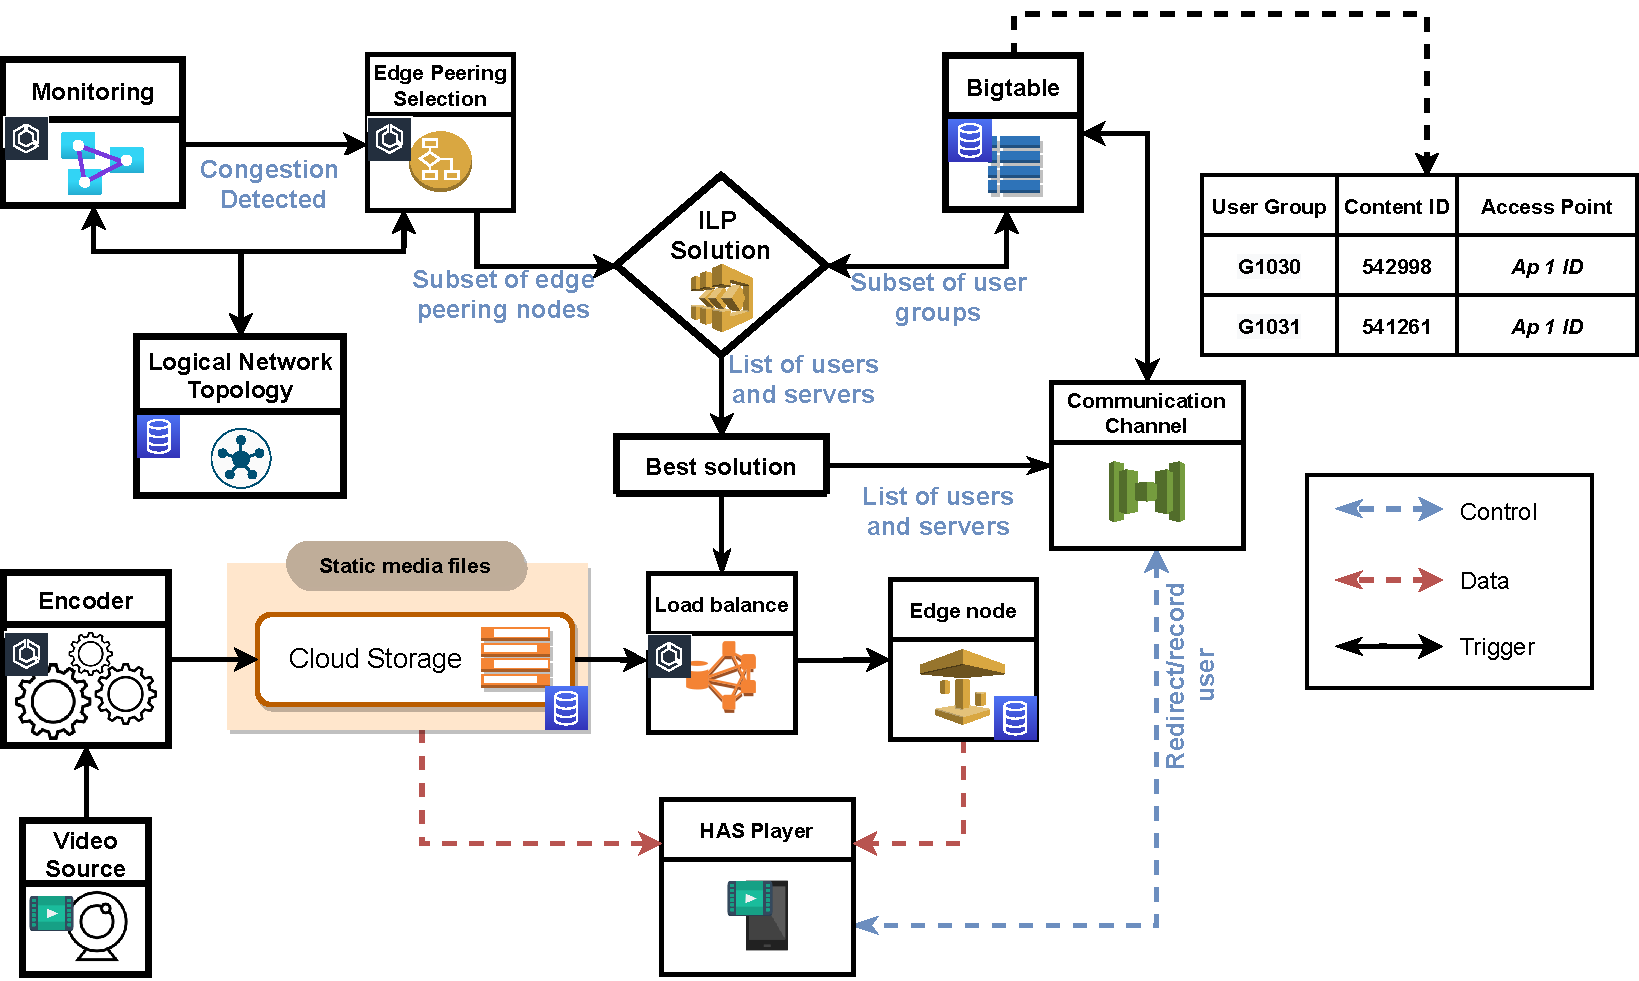
\includegraphics[width=\linewidth]{images/flow-model-infrastructure.pdf}
  \caption{Flowchart model of our proposed architecture.}
\end{figure}

As illustrated in Fig 2, we present the architecture system to perform all the requests/responses necessary for the streaming video service. The HAS client first requests the manifest to the server requests the manifest to the HTTP server. The dash player requests segments sequentially and dynamically adapts to network conditions using its adaptive bit rate (ABR) logic. ABR schemes also take into account playback buffering, device resources, viewer preferences, and content resources. Whereas the cloud storage is essentially an HTTP server that stores the chunks of different representations of various video content and the corresponding manifest files. In addition to the regular manifest files, the HAS server also stores the quality manifest files to list the perceptual qualities of the chunks. Below, we discuss the components in more detail.

\subsubsection*{Communication component}

The Communication Channel works as controller channel, in which the component is essential to realize the operation of communication with the cellular networks. The main class creates a control channel responsible of all communication between the entities. In this work, two communication functions are offered, \textit{i)} the redirection after the optimization component be performed, this way a triggered messages are activated to the users that will be redirected to other edge cache. Such message has to be sent after the server be available to the users start a HTTP connection. As second function offered, \textit{ii)} informations provided by the users, that includes various input variables (e.g., available bandwidth, congestion level, QoE, buffer level, device resolution, content type).
%the ID of the requested content and UE state data (e.g., buffer occupancy). 
The information also can assist the optimization module with periodical reports about the available BSs and their signal stregths. 

\subsubsection*{Tracking component}

The tracking component stores the player status at each step and keeps tracks of users' players. Before starting a streaming session, it first creates a logical network topology to group the HAS players into a set of virtual groups. Thereafter, each set of players whose belong to the same group are aggregated together into a common edge peering node using a simple aggregation (i.e., joint) function. If the user start requesting  the manifest, the already receive the server informatio updated, otherwise, and the user already whatching the video, a communication channel realizes this update. Thus helping to simplify processing and computation in the optimizer component.
%Second, it formulates the representation selection problem as a Partially Observable Markov Decision Process (POMDP) with various input variables (e.g., available bandwidth, congestion level, QoE, buffer level, device resolution, content type, subscription plan type), which represents our POMDP model abstraction consisting of three levels including players, clusters, and top-level POMDP model (aggregation of all players). Finally, at each step, the quality recommendation module manages and stores the per-cluster optimized decisions resulting from the solver, and then passes these outputs to the communication component.

\subsubsection*{Monitoring component}
In order to decide when adaptation is necessary, the system also needs to be aware of the current network conditions. Network monitoring is therefore required.
Therefore, the monitoring component observes the link bandwidth usage of logical network topology. The bandwith estimation is based on packet received/transmited of each network interface, the download speed over recent chuncks to be robust to bandwidth fluctuations. The monitoring module goal is to periodically estimates the throughput to fulfill the demand based on actual feedbacks and provisions a subset of servers to host the content. The monitoging module period $T$ is equal to a predefined value, here we are using 2s.

In order to estimate the throughput, monitoring module computes the number of packets received during each period $T$. The current audience estimated is defined as $s_{t}$. The estimated packet received at the next iteration $(t+T)$ is labeled $\widehat{s_{t+T}}$. Finally, $\Delta s$ represents the change in number of packets eceived, that is to say $\Delta s = s_{t} - s_{t-T}$. The module estimatess the throughput with the following formula:

$$
\widehat{s_{t+T}} = \frac{s_{t} + \Delta s}{T}
$$

As the actual replication is mostly based on clients feedbacks, a more accurate estimation is not required.

The throughput estimation uses the demand passing through $\widehat{s_{t+T}}$ to estimate how much throughput $D$ the overall system must provide to the users. Each client tries to reach a target quality (highest available video bitrate) $Q$. 
Besides, we introduce C, a dynamic corrective coefficient to address the network and server issues. It takes into account the mean average video bitrate $B (B \leqslant Q)$ displayed by all clients watching the stream and the failure rate $FR$, which is the portion of clients who failed to obtain in time the response of their last request from the server.

$$
C = \frac{Q}{B} * (1 + FR)
$$

The dynamic coefficient $C$ allows the system to scale according to current clients QoE. It is then possible to compute the required system Throughput that will be requested by the clients, using the following formula:

$$
D = C * \widehat{v_{t+T}} * (Q + O).
$$

\subsubsection*{Optimizer Component}

The optimizer component goal is to decide on the number of servers to minimize the required infrastructure scale but also to maximize the users' QoE. To do that, we divide time into two main classes, one class collect the inputs coming from monitoring and, em seguida, uma formalização em programação linear inteira (ILP) receive the input e procura maximizar the video content provisioning apresentada por redes multiniveis then, an integer linear programming (ILP) formalization receives the input and seeks to maximize the video content provisioning presented by multilevel networks. In the next section, through some experiments, it is possible to verify the impacts that occur in ABR decision mechanisms with a simple multilevel topology.
%the provision not only to answer end users throughput demand in video contents

Once the monitoring component detect a congested link, then the optimizer component is triggered. Firstly, the edge peering selection module is responsible to gathering the inputs coming from monitoring and bigtable, in which are a subset of the network topology containing the nodes below the congested link. By doing so, a subgroups with the best end-users are selected from this subnetwork topology. 

\begin{algorithm} \caption{Optimizer Component Algorithm}
\textbf{Input:}  \\
\hspace*{\algorithmicindent} $uP$, $cP$: List of user groups and edge nodes; \\
\textbf{Output:}  \\
\hspace*{\algorithmicindent} $G_{u}$: List of user groups to be redirected; \\
\hspace*{\algorithmicindent} $A$: List of edge peering nodes; \\
\begin{algorithmic}[1]
\State /* Phase 1: Pick user groups inside the network subset. */
\For{viewer group $i \in Groups$}
	\If{$i \notin G_{u}$ and $uP_{i} \cap F \neq \varnothing$}
		\State insert $i$ into $G_{u}$
	\EndIf
\EndFor \\

% \State Initilize $V(s) = 0$, for all $s \in \mathcal S^+$
\State /* Phase 2: cache Make Decision related to the allocation and media content. */ 
\State $A \leftarrow ILP Solution(G_{u}, F)$  \\ %edge peering servers from ILP model;	 \\

\State /* Phase 3: Offload Media Content tasks. */

\State $cP \leftarrow cP \cup A $
\For{server $i \in A$}
	\State Place Multimedia Service in edge server $i$;
	\If{$uP_{i} \neq A_{i}$}
		\State Insert $i$ into $cP$;
	\EndIf
\EndFor


\end{algorithmic}
\end{algorithm}

In algorithm [1] shows details of optimizer component, where $uP$ and $cP$ are the preferred list of edge nodes (by user groups) and the subset of of user groups, respectively.
To filter a subset of user groups, we first select the groups that rely on at least on node in $F$. Note that in practice, $F \cap uP_{i} \neq \varnothing$ is a subpath of the network topology. In Phase 2, we Make Decision related to the allocation and media content.

Next, we utilize the combined dataset to perform a solution in the ILP model.
% Path Selection and Resource Allocation
To support video services demanded by users, an optimal path set for all data flows should be found by solving the proposed algorithm. Denote $P_{i}$ as a path set including all candidate path for user $i$ and $P_{ij}$ as a subset of $P_{i}$ including all candidate paths starting from node $j$. A path $p_{ij}^{k} \in P_{i}$ means the $k-th$ path flow $i$ starting from node $j$ and the corresponding data rate of this path is denoted by $r_{ij}^{k}$ if $p_{ij}^{k}$ is selected.

%\subsection{Proposed ILP Solution}

To increase the number of attended by a single node, we use a Cost function $c_{ij}$. Where $\lambda_{i}$ is the number of users in group $i$ and $p_{j}$ is the probability that node $j$ can provide a video streaming for a number of users. 

\begin{equation}\label{cost_func}
c_{ij} = \lambda_{i} (1 - p_{j})
\end{equation}


To improve the whole network utility by maximizing the overall users' QoE, the controller performs traffic engineering to assist content provider selecting in real-time the best peering edge nodes to attend the end-users. Thus, the proposed problem can be formulated as follows.

Minimize
\begin{equation}
\sum^{G_u}_{i=1}\sum^{F}_{j=1} c_{ij}x_{ij} + \sum^{F}_{j=1} f_{j} y_{j} \label{eq:maximize}
\end{equation}

Subject to
\begin{equation}\label{bound_1}
\sum^{F}_{j=1} x_{ij} = 1 \text{ } \forall i \in G_u
\end{equation}
% \vspace{-0.3cm}
\begin{equation}\label{bound_3}
x_{ij} * d_{i}( bt_{i}^{max})
\leq Bw_{p_{ij}^{k}}
\text{ } \forall i \in G_u, j \in F; p_{ij}^{k} \in P_{ij} 
\end{equation}
\begin{equation}\label{bound_2}
\sum^{n}_{i=1} x_{ij} \leq M_{j}y_{j} \text{ } \forall j = 1,...,m
\end{equation}
% \vspace{-0.3cm}
% \begin{equation}\label{bound_4}
% x_{ij} \leq d_{i}y_{j} \text{ } \forall i = 1,...,n; \forall j = 1,...,m, 
% \end{equation}
% \vspace{-0.8cm}
\begin{equation}\label{bound_3}
x_{ij} \geq 0 \text{ } \forall i = 1,...,n; \forall j = 1,...,m
\end{equation}
% \vspace{-0.5cm}
\begin{equation}\label{bound_3}
y_{j} \in \{0,1\} \text{ } \forall j = 1,...,m
\end{equation}
\vspace{0.5cm}

The throughput estimation uses the demand passing through $\widehat{s_{t+T}}$ to estimate how much throughput $D$ the overall system must provide to the users. Each client tries to reach a target quality (highest available video bitrate) $Q$. 
Besides, we introduce C, a dynamic corrective coefficient to address the network and server issues. It takes into account the mean average video bitrate $B (B \leqslant Q)$ displayed by all clients watching the stream and the failure rate $FR$, which is the portion of clients who failed to obtain in time the response of their last request from the server.

\section{Modelling and Analysis of Cache Hierarchies}
\label{sec:mechanism}

We consider a cache hierarchies inside a edge/cloud networkrepresented as DAGs. The caches are triggered replacements at every cache which are activated to attend the users. This approximation is based on tracking an object hit at a parent cache back to a corresponding arrival.

\subsection{Decomposition Approach}

The overall goal of our design is to improve the QoE of content-downloading users, which is mainly characterized by the content latency and dontwnt download rate. To this end, our solutions for content caching and request scheduling strive to minimize the average content access delay and maximize the average content request rate in edge cache nodes, which are not always achieved simultaneously. Hence, an optimized tradeoff between the two objectives is targeted

Interestingly, content placement and request scheduling generally occur at different time scales: content popularity often varies slowly, at the scale of hours or days based on the measurement and prediction from various sources; on the other hand, request-scheduling decisions have to adapt to the dynamics in user location and channel conditions, which vary in the order of seconds. This makes a joint optimization to react promptly to the dynamic network changes difficult; hence, it motivates the decomposition of the overall problem into (i) the cache management subproblem, which takes the long-term content popularity as input, and (ii) the content request scheduling subproblem, which takes into account the incoming specific requests, the corresponding channel condition of the users, and the cache availability at the BSs and the CPU. Although the two subproblems are addressed separately due to their different time-scales, the coupling between the two is reflected by the fact that the solution of the cache-placement policy is used as input to the request scheduling policy. Likewise, the request-scheduling solution will affect the cache-placement decision the next time it is recalculated. This is because the content popularity is calculated based on the number of requests to each content at different BSs as the result of the request scheduling policy; hence, after a long-time-scale period (hours or days), the cache-placement decision will be made based on the updated content popularity

\subsection{Management Mechanism}

In this work, the client and server use the HTTP protocol at the application layer to perform all the necessary requests/responses. On the server side, once a media file~(or stream) is ready, it will be prepared for streaming before being published to a standard HTTP server. The original file/stream is partitioned into segments~(also called \textit{chunks}) of equivalent playtime, and multiple versions (also called representations) of each segment are generated that vary in bitrate/resolution/quality using an encoder or a transcoder.
In addition, the server generates a manifest file called a media presentation descriptor~(MPD), which lists the available representations, including information such as video timing, content availability, media types~(ie, H.264 , H.265, etc.), resolutions, minimum and maximum bandwidths, and the existence of several encoded alternatives of multimedia components, locations of media segments on the network, and other content characteristics.

On the HAS client side, first, the video player requests the manifest to the HTTP server and analyzes the information mentioned above. In this way, it can start requesting segments sequentially and dynamically adapt to network conditions using its bit rate adaptive logic~(ABR). ABR schemes also take into account playback buffer, device resources, viewer preferences, as well as content resources, with different weights.
Because the viewer's QoE needs to be determined in real-time during playback, objective metrics are often used, including the number of interruptions, duration of startup delay, frequency, and number of video quality flickers. By default, HAS does not require any specific adaptation scheme, leaving system developers to innovate and implement their own methods.

O controlador dentro do servidor CDN possui um canal de comunicação é criado com o usuário, assim as nossas mecanismos são capazes de se adaptar em tempo-real as necessidades da rede, bem como melhorar as

\begin{algorithm} \caption{Real-time Multimedia Management Mechanism}
\begin{algorithmic}[1]

% \State Initilize $V(s) = 0$, for all $s \in \mathcal S^+$

\State /* Phase 1: Make Decision related to the cache allocation and media content. */
\State Initialize $a_i = 0$, for all viewer $i \in M$;
\For {$i \in \textit{Grupos de usuários}$}
    \State $j \leftarrow \textup{head of } S_{i}$;
    \State Insert $i$ into $G_{j}$~($G_{j}^{k \cup i}$);
    \If{$D(G_{j}^{0 \sim k}) \leq C_{j}$}
        \State Label $G_{j}^{0 \sim k}$ with $j$;
    \EndIf
    % \State $v \gets V(s)$
    % \State $V(s) \gets \sum_a \pi(s,a) \sum_{s'} \mathcal P_{ss'}^a [ \mathcal R_{ss'}^a + \gamma V(s')$
    % \State $\Delta \gets \max(\Delta, |v- V(s)|)$
\EndFor

\State /* Phase 2: Redirecting viewers. */
\For{viewer i with ai = 0}
    \If{\textit{exists server} $j \in F$ \textit{with} $bd_j \geq b_i$ \textit{•}it{and} $s_i \in S_j$} 
        \State $a_i \gets j$; $bd_j \gets (bd_j - b_i)$;
    \EndIf 
\EndFor

\State /* Phase 3: Offload Media Content tasks. */

\Ensure $S_i$
\end{algorithmic}
\end{algorithm}


\section{References}

Bibliographic references must be unambiguous and uniform.  We recommend giving
the author names references in brackets, e.g. \cite{knuth:84},
\cite{boulic:91}, and \cite{smith:99}.

The references must be listed using 12 point font size, with 6 points of space
before each reference. The first line of each reference should not be
indented, while the subsequent should be indented by 0.5 cm.

\bibliographystyle{sbc}
\bibliography{sbc-template}

\end{document}
